\documentclass[14pt]{extarticle}
\usepackage{amsmath}
\usepackage{amssymb}
\usepackage{graphicx}
\usepackage{relsize}%
\graphicspath{ {../chap11/} }
\usepackage[top=1in, bottom=0.75in, left=0.75in, right=0.75in]{geometry}
\newcommand*{\Scale}[2][4]{\scalebox{#1}{\ensuremath{#2}}}%
\usepackage{hyperref}
\usepackage[most]{tcolorbox}
\definecolor{bg}{RGB}{255,249,227}


\begin{document}

\section*{Math 208 Discussion Outline for 12/10/2020}


\subsection{Homework and other due dates}
\begin{itemize}
\item Section 11.1 due 12/11
\item Section 11.2 due 12/15
\item Final Exam on 12/21, Monday at 10:00am to Noon. 
\end{itemize}

\subsection{Final Exam Procedures}
The Final will be done virtually on Collaborate Ultra. You will be required to have video ON while taking the exam, so make certain it will work for you beforehand.
\\\\
You will receive via email a link to your final exam session between 9:00am and 9:30am. Log into the session about 10 minutes prior to the scheduled time. You will then be given instructions and informed where to download the exam.
\\\\
During the exam, you must keep your camera on. Make sure you have a quiet location with a good Internet connection from which to work. If you have a question during the exam, raise your hand and I will visit your room and talk with you. Please understand that there will be about 60 other persons taking this exam simultaneously.
\\\\
You have about two hours to complete the exam. You will then have an extra 30 minutes, until 12:30PM, to convert your exam to a PDF and submit it via Canvas. Do not delay on this and if you have any problems contact me immediately. Late work will NOT be accepted.
\\\\
The submission deadline is 12:30PM.

\subsection{Section 11.2: Second Derivative and Graphs}
\subsubsection*{Understanding the graph and f''}
The second derivative, denoted by $f''(x) = \mathlarger{\frac{d^2y}{dx^2}}$ informs us of the concavity of the graph. It is equal to the derivative of the first derivative.
\\
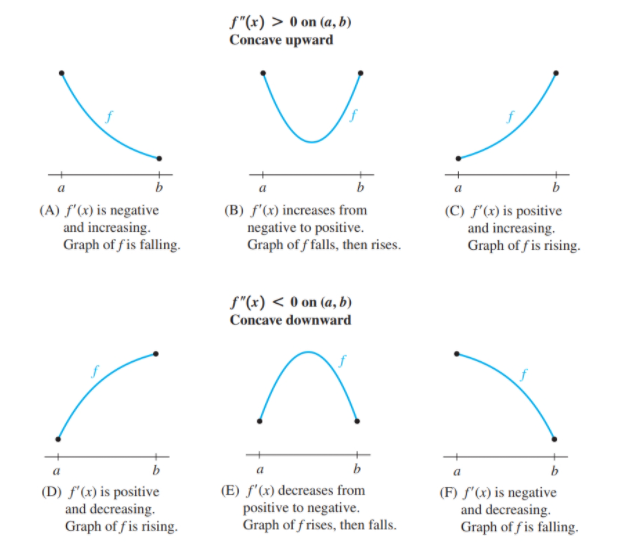
\includegraphics[width=0.9\linewidth]{11-2-1}


Just as with $f'$, interesting points happen when $f'' =0$. The book calls these partition numbers and it uses the sign chart to indicate them. An inflection point is a one of these interesting points on the graph if $f''(x_0)$ exists, the function is continuous at $x_0$, and the concavity changes at $x_0$.
\\
\\
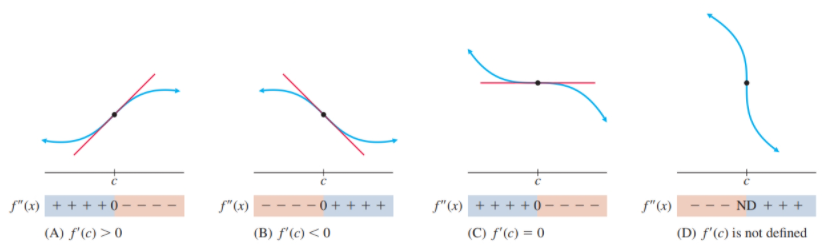
\includegraphics[width=1.0\linewidth]{11-2-2}
\\
\\
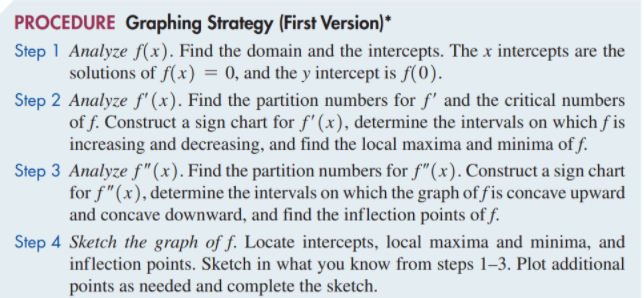
\includegraphics[width=0.9\linewidth]{11-2-3}

\subsubsection*{Examples}

Determine the sign charts for the first and second derivatives and indicate interesting points (max, min, inflection, and concavity).
\\
\begin{flalign*}
	&\text{(33) } f(x) = x^3 - 3x^2 + 7x+2 & \tag{Create and interpret sign chart}
\end{flalign*}
\begin{align*}
	f'(x)&= 3x^2 - 6x +7 \tag{When does f' = 0? $f' > 0$ for all x}\\
	f''(x) &= 6x - 6\tag{When does f'' = 0? Root at x=1.}\\
	f''(0) &=- 6\\
	f''(2) &= 6
\end{align*}

\begin{tabular}{|l|c|c|c|c|}
	\hline
	f &  &  &  &  \\
	\hline
	f' & +++ & +++ & +++ &  \\
	\hline
	f'' & - - - & 1 & +++ &  \\
	\hline
\end{tabular}
\\\\
Therefore $x = 1$ is an inflection point. It is concave down below $x<1$ and concave up for $x>1$.
\\
\vspace{1cm}
\\
\textbf{Full Example}: 
Summarize information in a sign chart and then graph the function $y=f(x)$.
\begin{flalign*}
	&\text{(61) } f(x) = (x^2 + 3)(9-x^2) & \tag{Create sign chart and graph}
\end{flalign*}
\begin{align*}
	f(x) &= -(x^2 + 3)(x^2-9) \tag{When does f equal 0?}\\
	&= -(x^2 + 3)(x+3)(x-3) \\
	&x = -3, x=3 \tag{Roots}\\
	f(-10) &<0 \\
	f(0) &>0 \\
	f(10) &<0
\end{align*}
\begin{align*}
	f'(x)&=-[2x(x^2-9) + (x^2+3)(2x)] \tag{When does f' equal 0?}\\
	&=-2x(x^2-9 + x^2+3) \\
	0 &=-4x(x^2-3) \\
	&x = 0, x=-\sqrt{3}, x=\sqrt{3} \tag{Roots}\\
	f'(-10) & = 40(97)>0 \\
	f'(-1) &= 4(-2)<0 \\
	f'(1) &=4(-2)>0 \\
	f'(10) &-40(97)<0
\end{align*}
\begin{align*}
	f'(x) &=-4x^3+12x \\
	f''(x) &=-12x^2 + 12 \tag{When does f' equal 0?}\\
	&=-12(x^2 - 1) \\
	&=-12(x+1)(x - 1) \\
	&x = -1, x=1 \tag{Roots}
	\\
	f''(-2) & = -48+12 <0 \\
	f''(0) &= 0 +12>0 \\
	f''(2) &=-48 + 12<0
\end{align*}
\begin{tabular}{|l|c|c|c|c|c|c|c|c|c|}
	\hline
	f & - - - & -3 & +++ & +++ & +++ & +++ & +++ & 3 & - - -  \\
	\hline
	f' & +++ & +++ & $-\sqrt{3}$ & - - - & 0 & +++ & $\sqrt{3}$ & - - - & - - - \\
	\hline
	f'' & - - - & - - - & - - - & -1 & +++ & 1 & - - - & - - - & - - - \\
	\hline
	f(x) & & 0 & 36 & 32 & 27 & 32 & 36 & 0 &  \\
	\hline
\end{tabular}

\subsubsection*{Homework}
31, 35, 57, 63, 65
\\
Extra Credit: Section 8.3 p 432 \# 18, 22, 48, 62, 78 (use Venn diagram)




\cleardoublepage

\end{document}
